Для всякой функции $u$, непрерывной вместе с первыми производными в замкнутой области $W$, ограниченной достаточно гладкой поверхностью $S$, и имеющей вторые производные внутри $W$, имеет место представление
\begin{equation}
	u(M_0) = \frac{1}{4 \pi} \iint\limits_{S} \left[ \frac{1}{R_{PA}} \derp{u}{n}{} - u(P) \derp{}{n}{} \left(\frac{1}{R_{PA}} \right) \right]\, d\sigma_p - \frac{1}{4 \pi} \iiint\limits_W \frac{\Delta u}{R_{MA}}\, d\tau_M.
\end{equation}

Если функция $u(A)$ гармоническая, то объёмный интеграл равен нулю; если же $u(A)$ удовлетворяет уравнению Пуассона, то объёмный интеграл является известной функцией.

Пусть $v(A)$ -- некоторая гармоническая функция, непрерывная в $W + S$ вместе с первыми производными, не имеющая нигде особенностей. Вторая формула Грина даёт
\begin{equation}
	0 = \iint\limits_S \left( v \derp{u}{n}{} - u \derp{v}{n}{} \right) \, d\sigma - \iiint\limits_W v \Delta u \, d \sigma
	\label{equ:equGreen2Trans}
\end{equation}

Складывая основную формулу Грина \eqref{equ:equMainGreen3d} и \eqref{equ:equGreen2Trans} получаем
\begin{equation}
	u(A) = \iint\limits_S \left[ G \derp{u}{n}{} - u \derp{G}{n}{}\right] \, d\sigma -  \iiint\limits_W \Delta u \cdot G \, d \tau
	\label{equ:equSourceFunction}
\end{equation}
где
\begin{equation}
	G(M, M_0) = \frac{1}{4 \pi R_{AP}} + v
	\label{equ:equSourceFunction2}
\end{equation}
-- функция двух точек. Точка $A$ фиксирована, и поэтому $x, y, z$ играют роль параметров.\\

Формула \eqref{equ:equSourceFunction} содержит $u\big|_S$ и $\left. \derp{u}{n}{} \right|_S$. При решении первой краевой задачи задаётся лишь $u\big|_S$, а при решении второй -- значение $\left. \derp{u}{n}{} \right|_S$. Функция $v$ выбирается таким образом, чтобы $G|_S = 0$ для первой краевой задачи $\left(\left. \derp{u}{n}{} \right|_S = 0 \: \mbox{для второй краевой задачи}\right)$. Определим функцию $G(A, P)$ при помощи условий:
\begin{enumerate}
	\item $G(A, P)$ как функция точки $P(\xi, \eta, \sigma)$ при фиксированной точке $A(x, y, z)$ удовлетворяет уравнению Лапласа
	\[
		\Delta G = G_{\xi \xi} + G_{\eta \eta} + G_{\sigma \sigma} = 0, \quad P \neq A
	\]
	во всех точках $P$ области $W$, кроме точки $P = A$.
	\item $G(A, P)$ при совпадении аргументов $(A = P)$ обращается в бесконечность и представима в виде \eqref{equ:equSourceFunction2}, где $v = v (A, P)$ -- гармоническая всюду в $W$ функция.
	\item $G(A, P)$ на границе обращается в нуль:
	\[
		G(A, P) = 0, \quad \mbox{если}\quad  P \in S
	\]
	Этому условию можно удовлетворить, потребовав, чтобы 
	\[
		v\big|_S = - \frac{1}{4 \pi R}
	\]
\end{enumerate}

Функцию $G$, определённую таким образом, будем называть \textit{функцией точечного источника первой краевой задачи для уравнения $\Delta u = 0$.} В самом деле, формула \eqref{equ:equSourceFunction} даёт:
\begin{equation}
	u(A) = - \iint\limits_S u \derp{G}{n}{}\, d\sigma = - \iint\limits_S f \derp{G}{n}{}\, d\sigma \quad (f = u\big|_s)
	\label{equ:equSourceFunction3}
\end{equation}
Формула \eqref{equ:equSourceFunction3} построена с помощью формулы Грина, предполагающей выполнение определённых условий в отношении функций $u$ и $G$ и поверхности $S$. В формулу  \eqref{equ:equSourceFunction3} входит выражение $\derp{G}{n}{}$, существование которого на поверхности $S$ не следует непосредственно из определения функции $G$.
%\[
%	\Delta u = 0 \quad u \in W
%\]
%\[
%	u|_s = f
%\]

%\[
%	W = \frac{1}{r_{AP}}
%\]
%где $
%	r_{AP} = \sqrt{(x - x_0)^2 + (y - y_0)^2 + (z - z_0)^2}
%$
%-- расстояние между точками $A(x, y, z)$ и $P (x_0, y_0, z_0)$.
%\begin{align*}
%	 &\derp{W}{x}{} = - \frac{1}{r_{AP}^2} \derp{r_{AP}}{x}{} = - \frac{1}{r_{AP}^2} \frac{2 (x - x_0)}{2 \sqrt{(x - x_0)^2 + (y - y_0)^2 + (z - z_0)^2}} = \frac{(x - x_0)}{r_{AP}^3}\\[10pt]
%	&\derp{W}{x}{2} = - \frac{1}{r_{AP}^3} + \frac{3 (x - x_0)^2}{r_{AP}^5}; \quad \derp{W}{y}{2} = - \frac{1}{r_{AP}^3} + \frac{3 (y - y_0)^2}{r_{AP}^5}; \quad \derp{W}{z}{2} = - \frac{1}{r_{AP}^3} + \frac{3 (z - z_0)^2}{r_{AP}^5}; 
%\end{align*}
%\[
%	\Delta u = - \frac{3}{r_{AP}^3} + \frac{3 [(x - x_0)^2 + (y - y_0)^2 + (z - z_0)^2]}{r_{AP}^5} = 0
%\]
%		Данное решение имеет в точке $A$ особенность.\\
%\[
%	\iint\limits_{S} \left(u \derp{v}{n}{} - v \derp{u}{n}{}\right) dS = \iint\limits_S \left(u \der{v}{n}{} - v \der{u}{n}{}\right) dS = \iiint\limits_{W} \left(u \Delta v - v \Delta u \right) d \omega
%\]
%		Решение $W = \frac{1}{r_{AP}}$ верно только в области $\omega$. Попробуем построить решение $W_1$ для всей области $W$.\\
%		
%		Построим функцию Грина\\
%\[
%	\Delta W_1 = 0 \quad W_1 |_S = W |_S
%\]
%\[
%	G (x, y, z, x_0, y_0, z_0) = W_1 - W; \quad G|_S = 0
%\]
%		Предположим, что в функции Грина $v = G$. Тогда 
%\[
%	\iint\limits_{S} \left(u \derp{v}{n}{} - v \derp{u}{n}{}\right) dS = \iint\limits_S \left(u \der{v}{n}{} - v \der{u}{n}{}\right) dS = \iiint\limits_{W} \left(u \Delta v - v \Delta u \right) d \omega
%\] %подписать что равно нулю
%\[
%	\iint\limits_{S} \left(u \derp{G}{n}{} \right) dS + \iint\limits_{S_1} \left(u \der{G}{n_1}{} - v \der{u}{n_1}{}\right) dS_1 = 0 
%\]
%		Перейдём к сферической системе координат.\\
%\begin{figure}[h!]
%	\centering
%	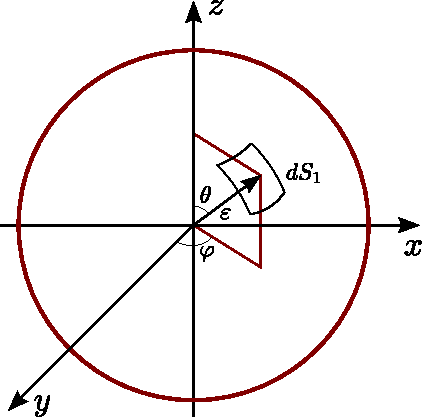
\includegraphics{figGreenIllust.pdf}
%\end{figure}
%\[
%	dS_1 = \varepsilon^2 \sin \theta \, dv d \varphi
%\]
%\[
%	\iint\limits_{S_1} \left(u \der{G}{n_1}{} - v \der{u}{n_1}{}\right) dS_1 = \int\limits_0^{2 \pi} d\varphi \int\limits_0^{\pi} \left(- u \der{G}{r}{} + G \der{u}{r}{} \right) \varepsilon \sin \theta d \theta
%\]

%\begin{multline*}
%	\lim\limits_{\varepsilon \to 0} \iint\limits_{S_1} \left( u \derp{G}{u_1}{} - G \derp{u}{u_1}{} \right) ds = - \int\limits_{0}^{2 \pi} d \varphi \int\limits_{0}^{\pi} d\theta \sin \theta u = \\ = u (x_0, y_0, z_0)\int\limits_0^{2 \pi} d \varphi \int\limits_{0}^{\pi} \sin \theta d \theta = - 4 \pi u (x_0, y_0, z_0) 
%\end{multline*}
%\[
%	u(x_0, y_0, z_0) = \frac{1}{4 \pi} \iint\limits_S f \derp{G}{u}{} dS
%\]
%Получили решение задачи Дирихле через функцию Грина.\\
%Функцию Грина можно построить для шара, сферы и полупространства.\\
